\documentclass[accentcolor=tud1c,colorback,ngerman,12pt] {tudreport}
\usepackage[utf8]{inputenc}
\usepackage{babel}
\usepackage{acronym}
\usepackage{listings}
\usepackage{tabularx}
\usepackage{url}
\usepackage{hyperref}

\lstset{language=C,basicstyle=\small, breaklines=true, showtabs=false, showspaces=false, showstringspaces=false}

\renewcommand{\lstlistingname}{Quelltext}
\lstset{literate=%
{Ö}{{\"O}}1
{Ä}{{\"A}}1
{Ü}{{\"U}}1
{ß}{{\ss}}1
{ü}{{\"u}}1
{ä}{{\"a}}1
{ö}{{\"o}}1
}

\setinstitutionlogo[height]{bilder/rechnersysteme-transparent}

\begin{document}
\title{Automatisches bauen und parallelisieren von Microblaze Systemen}
\subtitle{Masterthesis}
\subsubtitle{Christian Hohenbrink \hfill  \\4. Januar 2017}

\maketitle
\chapter*{Erklärung gemäß § 22 Abs. 7 APB}

Hiermit erkläre ich gemäß § 22 Abs. 7 der Allgemeinen Prüfungsbestimmungen (APB) der Technischen Universität Darmstadt in der Fassung der 4. Novelle vom 18. Juli 2012, dass ich die Arbeit selbstständig verfasst und alle genutzten Quellen angegeben habe und bestätige die Übereinstimmung von schriftlicher und elektronischer Fassung.\\ \\ \\ \\

\parbox{8cm}{\centering Darmstadt, den 4. Januar 2017\hrule
\strut \centering\footnotesize Ort, Datum} \hfill\parbox{8cm}{\phantom{Darmstadt, den 4. Januar 2017} \hrule
\strut \centering\footnotesize Name}

\vfill

\noindent \textbf{Fachbereich Elektro- und Informationstechnik}\\
Institut für Datentechnik\\
Fachgebiet Rechnersysteme\\
Prüfer: Prof. Dr.-Ing. Christian Hochberger\\
Betreuer: M.Sc. Kris Heid

\tableofcontents

\chapter{Einleitung}
\textit{kursiver Text} \\
\texttt{besonderer Text} \\
normaler Text
\begin{itemize}
\item[\textbf{1)}] \textbf{Aufzählung1}\\
Text der Aufzählung
\item [\textbf{2)}]\textbf{Aufzählung2}
\item [\textbf{3)}]\textbf{Aufzählung3}
\item [\textbf{4)}]\textbf{Aufzählung4}
\item [\textbf{5)}]\textbf{Aufzählung5}
\end{itemize}
Quellenverlinkung \cite{UCS_XDL_UseCaseSenarios}


\chapter{Grundlagen}
\section{SpartanMC Entwicklungsumgebung}
\subsection{JConfig}
JConfig ist der in Java programmierte Systembuilder der SpartanMC Entwicklungsumgebung. Mit ihm ist es möglich,
auf abstrakter Ebene ein System-on-Chip (SoC) zu beschreiben, welches für die Verwendung auf FPGAs bestimmt ist. \\
Bei der Erstellung einer neuen Konfiguration wird zunächst die Zielhardware festgelegt. JConfig generiert aus dieser
Angabe automatisch alle erforderlichen Optionen, die später von der ISE Toolchain benötigt werden, um ein Bitfile
zu generieren. Desweiteren können sämtliche Inputs und Outputs des SoC verwaltet werden (Einstellungen wie Spannungsniveau 
und Invertierung können vorgenommen werden).
Um ein SoC zu erstellen, können Hardwarekomponenten aus einer erweiterbaren Library ausgewählt werden. Ein IP-Core der
Library hinzuzufügt werden, indem zunächst Hardware Description Language (HDL) Dateien und eine Beschreibung des Cores in einem bestimmten Extensible Markup Language (XML) Format hinterlegt werden (siehe \ref{subsec:xml}).\\
Für jede Hardwarekomponente lassen sich sowohl Verbindungen zu anderen Komponenten, als auch Parameter definieren.
Speicherbausteine haben mit der Angabe eines Pfades zur verwendeten Firmware noch eine weitere Konfigurationsmöglichkeit.\\
Ist die Systembeschreibung abgeschlossen, können alle von der SpartanMC Toolchain benötigten Dateien generiert werden.
Dies umfasst eine Top-Level-Verilog-Beschreibung der Konfiguration, in der sämtliche IP-Cores instanziiert, parametrisiert und miteinander verbunden werden. Desweiteren werden Linkerskripte für die einzelnen Speicher angelegt und C-Headerdateien, die Informationen
über Modulparameter und Peripherien beinhalten und beim Schreiben der Firmware genutzt werden können. Ebenfalls erstellt werden
Makefiles, welche Konstanten definieren, die im weiteren Verlauf von der Maketoolchain verwendet werden. Es werden außerdem noch ein
User Constraints File (UCF) und Dateien erstellt, welche für die Simulation des SoC relevant sind.

\subsection{SpartanMC Toolchain}
Die SpartanMC Toolchain ist eine auf Makefiles basierende Toolchain, welche es dem Nutzer erlaubt, neue Projekte zu erstellen, diese zu
verwalten und den Workflow zu steuern. Durch die Makefiles ist es beispielsweise möglich, JConfig aufzurufen, ein Bitfile zu erstellen, welches
auf ein FPGA aufgespielt werden kann oder die Simulation zu starten. Alle relevanten Dateien, die zur Ausführung der Regeln in den Makefiles eines Projektes benötigt 
werden, werden von JConfig erzeugt (siehe vorheriger Abschnitt). Eine Ausnahme bildet die Firmware, welche der Nutzer selbst schreiben muss (die
Ordnerstruktur kann allerdings ebenfalls durch eine Make-Regel erzeugt werden).\\
Um ein Bitfile zu erstellen, verwendet die Toolchain die entsprechenden Tools aus der Xilinx ISE Design Suite. Die benötigten Steuerdaten und Kommandozeilenoptionen,
werden von JConfig erzeugt und in den Dateien \textit{project.mk}, \textit{spartanmc.xst} und \textit{spartanmc.prj} gespeichert.

\subsection{XML-Modulbeschreibung} \label{subsec:xml}
Um einen neuen IP-Core in JConfig nutzbar zu machen, ist es nötig eine XML-Modulbeschreibung zu erstellen. Hierzu sind in der SpartanMC Entwicklungsumgebung, unter dem Verzeichnis \textit{libdevxml}, XML Schema Definition (XSD) Dateien abgelegt, welche die Syntax für die verwendeten XML-Dateien
vorgibt.\\
Eine XML-Modulbeschreibung ist folgendermaßen gegliedert:
\begin{itemize}
\item \textbf{Header}: Im Header werden generelle Informationen angegeben, wie Kategorie und Name der Hardware.
\item \textbf{HDL}: In diesem Abschnitt wird angegeben, welche HDL-Dateien eingebunden werden sollen. Bei den Pfadangaben wird davon ausgegangen, dass sich die Dateien in einem Verzeichnis namens \textit{src} befinden, welches sich wiederum in dem Verzeichnis befindet, in dem die XML-Datei ist.
\item \textbf{Parameters}: Darauf folgen können mehrere Parameter-Abschnitte. Jeder einzelne Abschnitt wird im JConfig UI als eigene Gruppe in der Parametersektion dargestellt. Für Parameter lassen sich diverse Einstellungen treffen. So können Parameter beispielsweise über eine Auswahl von Werten definiert oder der Wertebereiche begrenzt werden.
\item \textbf{Ports}: Es können beliebig viele Ports-Abschnitte definiert werden. Dadurch wird die logische Zusammengehörigkeit der einzelnen Signale, die in einem jedem Abschnitt definiert sind, dargestellt. Einzelne Signale können mit einem Namen, Datenbreite und Richtung versehen werden.
\item \textbf{Bus}: Busse ermöglichen es Signale zusammenzufassen und somit das User Interface (UI) etwas übersichtlicher zu gestalten und den Arbeitsaufwand, um einzelne Signale zu verbinden, zu reduzieren.
\end{itemize} 
Außerdem gibt es noch einige besondere Konstrukte, welche nur für Module einer bestimmten Kategorie zur Verfügung stehen. Darunter fällt beispielsweise das \textit{addressLayout}, welches nur für Prozessoren relevant ist, um den Adressraum zu beschreiben oder \textit{memory}, welches nur für Speicherblöcke relevant ist.

\section{Xilinx Embedded Development Kit}
\subsection{Microblaze}
Der Microblaze von Xilinx ist ein für die Verwendung mit Xilinx FPGAs optimierter, 32-Bit Softcore Prozessor mit einer Reduced Instruction Set Computer (RISC) Architektur. Abbildung \ref{fig:MicroblazeBSB} zeigt das Blockschaltbild des Prozessors.\\
\begin{figure}[h!]
\centering
\includegraphics[width=1\linewidth]{./bilder/MicroblazeBSB}
\caption{Blockschaltbild des Microblaze \cite{MBREF}}
\label{fig:MicroblazeBSB}
\end{figure}
\noindent
Der Microblaze verfügt über 32 32-Bit breite general purpose Register, 32-Bit Instruktionen mit drei Operanden und zwei Adress-Modi, einen
32-Bit Addressbus sowie einer Single-Issue-Pipeline.\\
Neben diesen festen Eigenschaften ist der Microblaze über Parameter flexible konfigurierbar. So ist es beispielsweise möglich, über den Parameter C\_AREA\_OPTIMIZED die Anzahl der Pipelinestufen auf drei oder fünf festzulegen. Weitere Features des Microblaze sind in folgender Liste dargestellt:\\
\begin{itemize}
\item \textbf{Hardwarebeschleuniger}: Dem Microblaze steht dedizierte Hardware für verschieden Aufgaben zur Verfügung, die bei Bedarf per Parameter hinzugefügt werden. Dazu zählen ein Integer Dividierer, ein Integer Multiplizier, eine Floating Point Unit (FPU) und ein Barrel Shifter. In der Instruction Set Architecture (ISA) sind für die Hardwarebeschleuniger eigene Instruktionen vorgesehen (z.b. fmul für eine Gleitkomma Multiplikation).
\item \textbf{MMU}: Der Microblaze verfügt über eine konfigurierbare Memory Management Unit (MMU). Dabei stehen drei verschiedene Modi zur Verfügung: Usermode, Protection und Virtual. Außerdem verfügt die MMU über je einen Translation Lookaside Buffer (TLB) für Instruktionen und für Daten.
\item \textbf{Caches}: Werden externe Speicher verwendet, kann der Microblaze auf Caches sowohl für Instruktionen, als auch für Daten zurückgreifen. Hierbei lassen sich Einstellungen wie Größe des Caches, Länge einer Cacheline und Datenbreite festlegen.
\item \textbf{Speicher- und I/O-Zugriff}: Der Microblaze hat für Speicher- und I/O-Zugriffe verschiedene Möglichkeiten. Einerseits existiert der Local Memory Bus (LMB), ein Bus mit geringer Latenz, welcher für Zugriffe auf On-Chip Speicherblöcke gedacht ist. Das Advanced eXtensible Interface (AXI4) und der Processor Local Bus (PLB) sind sowohl für Speicher- als auch für I/O-Zugriffe nutzbar.
Das Xilinx CacheLink (XCL) Interface ist als hochperformante Lösung für Zugriffe auf externe Speicher gedacht. Voraussetzung für die Nutzung ist, dass der Memory Controller, an den das XCL Interface angeschlossen ist, FSL-Buffer implementiert.
\item \textbf{Debugging}: Der Microblaze verfügt ebenfalls über die Möglichkeit zum Hardware Debugging, es wird allerdings ein zusätzliches externes Debugging-Modul benötigt.
\item \textbf{Streaming Interfaces}: Um Daten mit geringem Overhead zu übertragen, verfügt der Microblaze über die Streaming Interfaces AXI4-Stream und FSL. Für FSL muss ein Buffer zur Verfügung stehen, um versendete Daten zu puffern.
\item \textbf{Exceptions}: Der Microblaze kann so konfiguriert werden, dass bei bestimmten Ereignissen (z.b. Math Exceptions, Bus Exceptions, ...) Hardware Exceptions ausgelöst werden.
\end{itemize}
Für weitere Informationen kann das Handbuch des Microblaze zu Rate gezogen werden (\cite{MBREF} \textit{Kapitel 2 - Microblaze Architecture}).
\subsection{XPS}
Das Xilinx Platform Studio (XPS) ist der Systembuilder von Xilinx. Mit ihm lassen sich per grafischer Oberfläche SoC erstellen. Über einen Wizard kann zu Beginn ein Basis-System erstellt werden, welches sich danach einfach erweitern lässt. Aus einem Katalog von IP-Cores kann zusätzliche Hardware ausgewählt werden, welche dann über einen Wizard konfiguriert werden kann. Desweiteren bietet XPS einfache Möglichkeiten, Komponenten untereinander zu verbinden, Adressen von I/O und Speicherblöcken anzupassen und Eingangs- und Ausgangssignale zu verwalten. Außerdem ist es möglich, von der Nutzeroberfläche eine Netzliste zu generieren oder das Hardwaredesign (inklusive Bitfile) zum Software Development Kit (SDK) zu exportieren, um Code für das SoC zu schreiben. \cite{MBTOOLS}
\subsection{SDK}
Mit dem SDK ist es möglich, Software für den Microblaze zu erstellen. Basierend auf der exportierten Hardware kann das SDK ein Board Support Package (BSP) erstellen, welches alle relevanten Treiber einbindet. Desweiteren lassen sich über Templates schnell einfache Beispielprogramme erstellen. Dem Softwareprojekt ist eine Makefile Struktur hinterlegt, die bei Änderungen an dem Source Code relevante Teile neu kompiliert. Außerdem ist es möglich, das FPGA mit dem aktualisierten Bitfile zu programmieren und auch zu debuggen. \cite{MBTOOLS}

\subsection{FSL}
FSL ist eine unidirektionale Punkt-zu-Punkt Verbindung die eine einfache und schnelle Datenübertragung zwischen Hardware, die das FSL-Interface implementiert, ermöglicht. Xilinx bietet als Implementierung eines FSL-Buses den \textit{FSL V20 Bus} IP-Core an \cite{FSL_CORE}. Diese Hardware bietet eine auf First-In-First-Out (FIFO) Speichern basierte Kommunikation. Abbildung \ref{fig:FSLBSB} zeigt das Blockschaltbild der FSL-Bus Komponente.

\begin{figure}[th!]
\centering
\includegraphics[width=0.7\linewidth]{./bilder/FSLBSB}
\caption{Blockschaltbild des Xilinx FSL IP-Cores \cite{FSL_CORE}}
\label{fig:FSLBSB}
\end{figure}
\noindent
Der Bus kann entweder synchron oder asynchron betrieben werden. Für den asynchronen Betrieb stellen Master und Slave eigene Taktsignale zur Verfügung (\textit{FSL\_M\_Clk} und \textit{FSL\_S\_Clk}), für den synchronen Betrieb wird ein globales Signal verwendet, welches nicht im Blockschaltbild dargestellt ist.\\
Um Daten in den FIFO-Speicher zu schreiben, muss der Master das \textit{FSL\_M\_Write}-Signal anlegen. Dies ist allerdings nur dann möglich, wenn das \textit{FSL\_M\_Full}-Signal anzeigt, dass der Speicher nicht voll ist. Neben einfachen Nutzdaten kann außerdem ein Steuerbit übertragen werden, welches beispielsweise dazu genutzt werden kann, um zwischen Steuer- und Nutzdaten zu unterscheiden. Der Slave wiederum kann Daten aus dem Speicher lesen, insofern das \textit{FSL\_S\_Exists}-Signal gesetzt ist.\\
Für den IP-Core können des weiteren noch Einstellungen über Implementationsart der FIFO-Speicher (Block Random Access Memory (RAM) oder Look Up Table (LUT) RAM), Tiefe des FIFO-Speichers oder Art des Taktmodus (synchron oder asynchron) getroffen werden. Für genauere Informationen zu Signalen, Parametern und Buszugriffen, kann das Datenblatt des IP-Cores zu Rate gezogen werden \cite{FSL_CORE}.\\
In der ISA des Microblaze sind mit \textit{get}, \textit{getd}, \textit{put} und \textit{putd} besondere Instruktionen vorhanden, die es ermöglichen, Daten direkt vom Registersatz über das FSL-Interface zu schreiben, bzw. Daten vom FSL-Interface direkt in den Registersatz einzulesen. Dies ermöglicht Übertragungen mit niedriger Latenz.
\subsection{Speicherinitialisierung im Microblaze} \label{subsec:MemInitBMM}
Für die Speicherinitialisierung im Microblaze stellt Xilinx das Tool data2mem zur Verfügung. \cite{DATA2MEM}
Data2mem liest sowohl eine textuelle Beschreibung der Speicherarchitektur in Form von Block RAM Memory Map (BMM) Dateien ein, als auch ausführbaren Code in Form von Executable and Linkable Format (ELF) Dateien. Mit diesen Dateien als Input ist es möglich, Speicherinitialisierungen in Form von UCF, Verilog oder Very High Speed Integrated Circuit Hardware Description Language (VHDL) Dateien zu erzeugen, die während der Synthese (UCF Datei) oder Simulation (HDL Dateien) verwendet werden können. Desweiteren ist es möglich, Block RAMs in existierenden Bitfiles zu aktualisieren, ohne den kompletten Toolflow noch einmal durchlaufen zu müssen.\\
BMM-Dateien haben eine eigene Syntax, die anhand des folgenden Ausschnitts einer BMM Datei erklärt wird.
\newpage
\begin{lstlisting}
ADDRESS_MAP microblaze_spmc_0 MICROBLAZE-LE 1
	ADDRESS_SPACE microblaze_spmc_0_bram_block_combined COMBINED [0x0:0x1fff]
		ADDRESS_RANGE RAMB16
		BUS_BLOCK
			microblaze_spmc_0_microblaze_mem_local_0/mem_core/MEM_BL[0].DPRAM [31:24];
			microblaze_spmc_0_microblaze_mem_local_0/mem_core/MEM_BL[1].DPRAM [23:16];
			microblaze_spmc_0_microblaze_mem_local_0/mem_core/MEM_BL[2].DPRAM [15:8];
			microblaze_spmc_0_microblaze_mem_local_0/mem_core/MEM_BL[3].DPRAM [7:0];
		END_BUS_BLOCK;
		END_ADDRESS_RANGE;
	END_ADDRESS_SPACE;
END_ADDRESS_MAP;
\end{lstlisting}
\textit{ADDRESS\_MAP} definiert die Speicherabbildung für einen bestimmten Prozessor mit dem Namen \textit{microblaze\_spmc\_0} vom Prozessortyp MICROBLAZE-LE mit der Prozessor ID 1. Es können beliebig viele \textit{ADDRESS\_MAP}-Blöcke hinzugefügt werden.\\ \textit{ADDRESS\_SPACE} definiert einen kontinuierlichen Speicherbereich des entsprechenden Prozessors. Innerhalb eines \textit{ADDRESS\_SPACE}-Abschnitts können mehrere \textit{ADDRESS\_RANGE}-Blöcke vorkommen. Jeder dieser Blöcke beschreibt einen Speicherbereich, mit einer Größe die einer Potenz von Zwei entspricht. So lassen sich auch asymetrische Speicherstrukturen beschreiben.\\
In einem \textit{BUS\_BLOCK}-Abschnitt wird beschrieben, wie viele Bitlanes der Speicher hat und welchem Block RAM welche Bitlane zugewiesen ist.
\chapter{Konzeption und Implementation}
\section{Anforderungen}
Ziel dieser Arbeit ist es, den Xilinx Microblaze in die bestehende SpartanMC Entwicklungsumgebung zu integrieren. Um dies zu erreichen, muss zunächst der Microblaze in JConfig eingebunden werden. Der CoreGenerator von Xilinx bietet keine Alternative, da lediglich das Microblaze Micro Controller System (MCS) \cite{MCS} zur Verfügung steht. Dies ist ein System bestehend aus einem Microblaze, Speicher und grundlegenden Peripherien, wie einem UART-Core und Timern. Die Konfigurierbarkeit des Microblaze innerhalb des MCS ist stark eingeschränkt. Features wie Caches oder FSL-Interface stehen nicht zur Verfügung und die Pipeline ist immer dreistufig. Da auf die umfangreiche Konfigurierbarkeit und das FSL-Interface nicht verzichtet werden soll, muss der Microblaze in JConfig integriert werden. Um dies zu erreichen, müssen zunächst sowohl eine Hardwarebeschreibung, als auch eine XML-Modulbeschreibung für den Microblaze erstellt werden. Dies ist ebenso erforderlich für den UART IP-Core und den FSL-Bus IP-Core. Bei der Erstellung der Hardware- und der XML-Modulbeschreibung, ist darauf zu achten, dass dem Nutzer es ermöglicht wird, die Parameter der neuen Komponenten konfigurieren zu können.\\
Es ist außerdem erforderlich, dass Anpassungen an der SpartanMC Toolchain vorgenommen werden. Dies ist notwendig, um die automatische Speicherinitialisierung für den Microblaze zu ermöglichen, da die bestehende Methode der Speicherinitialisierung für den SpartanMC nicht ohne Änderungen für den Microblaze anwendbar ist. Desweiteren muss der Compiler für den Microblaze in die Toolchain integriert werden, da einige der Hardwarebeschleuniger über spezielle Instruktionen angesprochen werden. Eine Vielzahl von IP-Cores von Xilinx sind in VHDL verfasst. Da in der SpartanMC Entwicklungsumgebung IP-Cores zum Großteil in Verilog verfasst wurden, ist es gegebenfalls notwendig, Anpassungen an der Toolchain vorzunehmen, um VHDL Designs zu unterstützen.\\
Optional wäre es wünschenswert, die erfolgreiche Paralellisierung eines Microblaze Programms durch \textmu\/Streams zu zeigen. Hierzu wäre es notwendig, 
\textmu\/Streams soweit anzupassen, dass eine entsprechende Hardwarekonfiguration mit den neu integrierten Komponenten erstellt werden kann und
die Aufrufe der Core-Konnektoren durch Aufrufe der FSL-Blöcke ersetzt werden.
\section{Integration in JConfig}
\subsection{Hardware}
Bevor über die Integration nachgedacht werden kann, muss zunächst festgelegt werden, welche Hardware verwendet wird. Über die Jahre hat Xilinx diverse Versionen des Microblaze veröffentlicht. Die Implementationen des Prozessors sind allesamt verschlüsselt und können nur mit entsprechendem Key entschlüsselt werden. Mit der Einführung von Vivado und der Einstellung der Entwicklung von ISE, änderte sich auch die Art der Verschlüsselung, sodass neuere Versionen des Microblaze nicht mehr von der alten Toolchain entschlüsselt werden können. Da die JConfig Toolchain allerdings Gebrauch von der ISE Toolchain macht, kommen für diese Arbeit nur der Microblaze v8.50c oder ältere Versionen in Frage.\\
Ausgehend vom ISE Installationsverzeichnis, ist das Verzeichnis für die IP-Cores an folgender Stelle zu finden: \textit{"14.7/ISE\_DS/EDK/hw/XilinxProcessorIPLib/pcores/"}. Dort sind alle Versionen des Microblaze, sowie alle Versionen der restlichen Hardware abgelegt. Für sämtliche verwendete IP-Cores werden die aktuellsten Versionen verwendet.
\subsection{Hardwarebeschreibung}
\subsubsection{Erzeugung der Hardwarebeschreibung mit XPS}
Um den Microblaze in JConfig integrieren zu können, ist es zunächst notwendig, eine Hardwarebeschreibung zu erstellen, die den Microblaze instanziiert und parametrisiert.
Diese kann entweder manuell erstellt werden oder mit XPS. In XPS kann dazu mit dem Base-System-Builder ein einfaches System erzeugt werden. Ein Beispiel für ein System ohne Peripherie ist in Abbildung \ref{fig:XPS_EXAMPLE} zu sehen.
\begin{figure}[ht!]
\centering
\includegraphics[width=1\linewidth]{./bilder/XPS_EXAMPLE}
\caption{Einfaches mit XPS generiertes System ohne Peripherie}
\label{fig:XPS_EXAMPLE}
\end{figure}
Das System besteht aus einem Micorblaze, zwei LMB, zwei Speichercontrollern (je einen für Daten und einen für Instruktionen), einem Block RAM als Programm- und Datenspeicher, einem AXI4-Light-Bus zur Anbindung von Peripherie, einem Reset-Core, einem Taktgenerator und einem Debug Modul. Um die Komplexität des Systems und somit zusätzliche Fehlerquellen zu reduzieren, werden der AXI4-Light-Bus, der Taktgenerator und das Debug Modul zunächst entfernt. Der AXI4-Bus wird nicht benötigt, da es zunächst in der SpartanMC Entwicklungsumgebung mit dem UART IP-Core nur eine Peripherie geben wird und diese direkt mit dem Prozessor verbunden werden kann. Der Taktgenerator wird nicht benötigt, da JConfig bereits über eigene Taktgeneratoren verfügt und das Debug Modul wird nicht benötigt, um die grundsätzliche Lauffähigkeit eines Microblaze Systems zu gewährleisten, sondern nur um Softwareanwendungen zu debuggen.\\
Nun kann in XPS eine Netzliste erzeugt werden. Als Nebenprodukt werden Wrapperdateien erstellt, die die einzelnen Komponenten mit den, im XPS angegebenen Einstellungen instanziieren. Die erzeugten Dateien werden nach Möglichkeit in der präferierten Sprache erzeugt, allerdings funktioniert dies bei manchen Wrapper Dateien nicht und sie werden in VHDL generiert. Die Top-Level-Beschreibung, welche sämtliche Komponenten instanziiert und miteinander verbindet, kann allerdings auch in Verilog erzeugt werden. Desweiteren besitzt die Top-Level-Beschreibung lediglich die, im XPS als extern makierten Signale als Eingänge und Ausgänge. Die Wrapper Datei für das Block RAM stellt eine Besonderheit dar. Für das Block RAM wird nämlich, entsprechend der angegebenen Größe des Speichers, ein elaboriertes Modell erzeugt. Dieses Modell funktioniert nur für die angegebene Speichergröße und lässt sich ohne großen Aufwand auch nicht ändern. Als Lösung des Problems wird ein generisches Speichermodul in Verilog geschrieben, welches das Verhalten der elaborierten Blöcke nachahmt (siehe \ref{subsubsec:genMem}).\\
Um nun eine konfigurierbare Hardwarebeschreibung zu erhalten, ist es notwendig, den Wrapperdateien und der Top-Level-Beschreibung Parameter hinzuzufügen. So können bei der Instanziierung des Top-Level-Moduls Parameter übergeben werden, die dann wiederum bei der Instanziierung der einzelnen Komponenten des Systems an diese weitergegeben werden können. Ebenso ist es erforderlich, dass Signale die verwendet werden sollen, als Eingänge bzw. Ausgänge der Top-Level-Beschreibung hinzugefügt und über Signale mit der entsprechenden Komponente verbunden werden. Für den Microblaze sind dies zu Beginn, neben Takt- und Reset-Signalen, Signale für den Programm- und Datenspeicher, AXI4-Signale und Signale, die dem FSL-Interface zuzuschreiben sind.\\
Unter Berücksichtigung der XML-Modulbeschreibung, ist es notwendig, den Speicher als externes Modul zu handhaben, da die XML-Syntax für Prozessoren keine integrierten Speicher unterstützt. Hierzu werden die Speichercontroller und das Block RAM in einem weiteren Modul zusammengefasst (siehe \ref{subsubsec:genMem}), sodass das Modul für den Microblaze noch aus den Instanzen für den Microblaze selbst, den beiden LMB und dem Reset-Core besteht. Die LMB-Cores erlauben es mehr als einen Speicher an den Microblaze anzuschließen.\\
Welche Parameter für die Konfiguration des Microblaze wichtig sind, wird im nächsten Abschnitt behandelt. 
\subsubsection{Handhabung der Parameter}
In diesem Kapitel wird behandelt, welche Parameter für die Konfiguration des Microblaze-Systems wichtig sind.
Für die Parameter des Microblaze wird die Tabelle aus dem Abschnitt \textit{MicroBlaze Core Configurability} in Kapitel 3 des Microblaze Datenblattes \cite{MBREF} herangezogen. Parameter, die in der Tabelle nur einen Wert in der Spalte \textit{Allowable Values} haben, werden fest auf diesen Wert gesetzt und können nicht vom Anwender verändert werden. In der Tabelle \ref{tab:MicParam} werden lediglich die Parameter behandelt, welche mehr als einen erlaubten Wert haben, allerdings trotzdem auf einen festen Wert gesetzt werden. Alle anderen Parameter, die nicht genannt werden, stehen dem Nutzer zur freien Konfiguration zur Verfügung. Erklärungen zu den Bedeutungen der einzelnen Parametern werden in Kurzform in der XML-Modulbeschreibung hinterlegt, sodass der Nutzer während der Erstellung eines Systems weiß, welche Funktion die einzelnen Parameter haben. Für detailliert Beschreibungen sei noch einmal auf das Datenblatt des Microblaze verwiesen \cite{MBREF}.
\begin{table}[ht!]
	\begin{tabular}{|l|c|p{10cm}|}
		\hline \textbf{Parameter} & \textbf{Wert} & \textbf{Beschreibung} \\ 
		\hline C\_LOCKSTEP\_SLAVE & 0 & Im Lockstep Modus können zwei oder mehrere \newline Microblaze das selbe Programm ausführen und die Ergebnisse miteinander vergleichen, um Hardwarefehler zu erkennen. Wird nicht benötigt.\\ 
		\hline C\_ENDIANNESS & 1 & Endianness wird auf Little Endian festgelegt. In XPS lässt sich dieser Wert nicht manuell verändern, dementsprechend wird auch unter JConfig darauf verzichtet.\\ 
		\hline C\_D\_AXI & 1 & Das AXI-Daten-Interface kann verwendet werden. \\ 
		\hline C\_I\_AXI & 1 & Das AXI-Instruktionen-Interface kann verwendet werden. (Nützlich bei externen Speicher) \\ 
		\hline C\_D\_PLB & 0 & Da bereits AXI verwendet wird, wird der PLB Bus nicht gebraucht und deshalb deaktiviert. \\ 
		\hline C\_I\_PLB & 0 & Siehe vorheriger Eintrag. \\ 
		\hline C\_D\_LMB & 1 & Das LMB-Daten-Interface kann verwendet werden. \\ 
		\hline C\_I\_LMB & 1 & Das LMB-Instruktionen-Interface kann verwendet werden. \\ 
		\hline C\_IPLB\_BUS\_EXCEPTION & 0 & Da der PLB nicht verwendet wird, werden die Exceptions auch nicht benötigt. \\ 
		\hline C\_DPLB\_BUS\_EXCEPTION & 0 & Siehe vorheriger Eintrag. \\ 
		\hline C\_ADDR\_TAG\_BITS & 17 & Das Datenblatt gibt kaum nützliche Informationen zu diesem Parameter, daher wird er auf den Default-Wert festgesetzt. \\ 
		\hline C\_DCACHE\_ADDR\_TAG & 17 & Siehe vorheriger Eintrag. \\ 
		\hline C\_USE\_EXT\_BRK & 0 & Siehe vorheriger Eintrag. \\ 
		\hline C\_USE\_EXT\_NM\_BRK & 0 & Siehe vorheriger Eintrag. \\ 
		\hline 
	\end{tabular}
	\centering
	\caption{Parameter des Microblaze die mehr als einen erlaubten Wert haben, aber dennoch auf einen Wert festegelegt werden.}
	\label{tab:MicParam}
\end{table}
Neben dem Microblaze werden mit einem generischen Speichermodul, einem UART-Modul und einem FSL-Modul noch drei weitere Hardwarekomponenten für JConfig erstellt, die parametrisiert werden können. Welche Parameter zur Verfügung stehen und was diese bewirken, ist in den Tabellen \ref{tab:MemParam}, \ref{tab:UARTParam} und \ref{tab:FSLParam} aufgeführt.

\begin{table}[ht!]
	\begin{tabular}{|l|p{10cm}|}
		\hline \textbf{Parameter} & \textbf{Beschreibung} \\ 
		\hline C\_FAMILY & Dieser Parameter wird von Xilinx IP-Cores verwendet, um, je nach verwendeter Hardware, vorhandene Primitives zu instanziieren. \\ 
		\hline RAMBLOCKS & Ähnlich wie für den Speicher des SpartanMC, kann angegeben werden, wie viel RAM instanziiert werden soll. Ein Block ist jeweils 2KB groß. Es können nur Größen gewählt werden, die einer Potenz von Zwei entsprechen, da mit jeder Vergrößerung des Speichers sich die Anzahl der Bitlanes verdoppelt.\\ 
		\hline C\_BASEADDRESS & Gibt die Startaddresse des Speichers an.\\ 
		\hline 
	\end{tabular}
	\centering
	\caption{Parameter des Speichermoduls für den Microblaze.}
	\label{tab:MemParam}
\end{table}

\begin{table}[ht!]
	\begin{tabular}{|l|p{10cm}|}
		\hline \textbf{Parameter} & \textbf{Beschreibung} \\ 
		\hline C\_S\_AXI\_ACLK\_FREQ\_HZ & Frequenz des Taktsignals, welches automatisch aus dem Takt abgeleitet wird.\\ 
		\hline C\_FAMILY & Dieser Parameter wird von Xilinx IP-Cores verwendet, um, je nach verwendeter Hardware, vorhandene Primitives zu instanziieren.\\ 
		\hline C\_BAUDRATE & Für die Übertragung verwendete Baudrate. Eine Auswahl von Werten zwischen 110 und 921600 steht zur Verfügung. \\ 
		\hline C\_DATABITS & Anzahl der zu übertragenden Bits pro Frame. Werte von 5 bis 8 sind möglich. \\ 
		\hline C\_USE\_PARITY & Gibt an, ob ein Paritätsbit mit übertragen wird. \\ 
		\hline C\_ODD\_PARITY & Gibt an, ob die Parität gerade oder ungerade ist. \\ 
		\hline 
	\end{tabular}
	\centering
	\caption{Parameter des UART-Cores.}
	\label{tab:UARTParam}
\end{table}

\begin{table}[ht!]
	\begin{tabular}{|l|p{10cm}|}
		\hline \textbf{Parameter} & \textbf{Beschreibung} \\ 
		\hline C\_EXT\_RESET\_HIGH & Gibt an, ob das externe Reset-Signal high-aktiv oder low-aktiv ist.\\ 
		\hline C\_ASYNC\_CLKS & Gibt an, ob das FSL-Interface synchron oder asyncron betrieben werden soll.\\ 
		\hline C\_IMPL\_STYLE & Wenn dieser Parameter auf 0 gesetzt ist, wird der FIFO-Speicher mit LUT RAMs implementiert, andernfalls mit Block RAMs.   \\ 
		\hline C\_USE\_CONTROLL & Bestimmt, ob das Steuerbit mit übertragen wird oder nicht.\\ 
		\hline C\_FSL\_DWIDTH & Ist auf 32 Bit festgelegt, da andere Datenbreiten im Zusammenhang mit dem Microblaze wenig sinnvoll sind. \\ 
		\hline C\_FSL\_DEPTH & Beschreibt die Größe des FIFO-Speichers. Diese ist von den Parametern C\_ASYNC\_CLKS und C\_IMPL\_STYLE abhängig. C\_ASYNC\_CLKS=0 => 1-8192. C\_ASNYNC\_CLKS=1 und C\_IMPL\_STYLE=0 => 16-128. C\_ASNYNC\_CLKS=1 und C\_IMPL\_STYLE=1 => 512-8192. Ist C\_ASNYNC\_CLKS=1 muss die Größe außerdem einer Potenz von Zwei entsprechen.\\ 
		\hline C\_READ\_CLOCK\_PERIOD & Wird automatisch aus dem Taktsignal berechnet. Wird genutzt um Timing Constraints für den asynchronen Pfad durch LUT RAMs zu erzuegen \\
		\hline 
	\end{tabular}
	\centering
	\caption{Parameter des FSL-Cores.}
	\label{tab:FSLParam}
\end{table}

\subsubsection{Implementation eines generischen Speichermoduls} \label{subsubsec:genMem}
Bevor über eine Implementation eines generischen Speichermoduls nachgedacht werden kann, sollte zunächst die Struktur, des von Xilinx verwendeten Speichers erläutert werden. Hierzu wird Abbildung \ref{fig:XilinxMEM} herangezogen.
\begin{figure}[ht!]
\centering
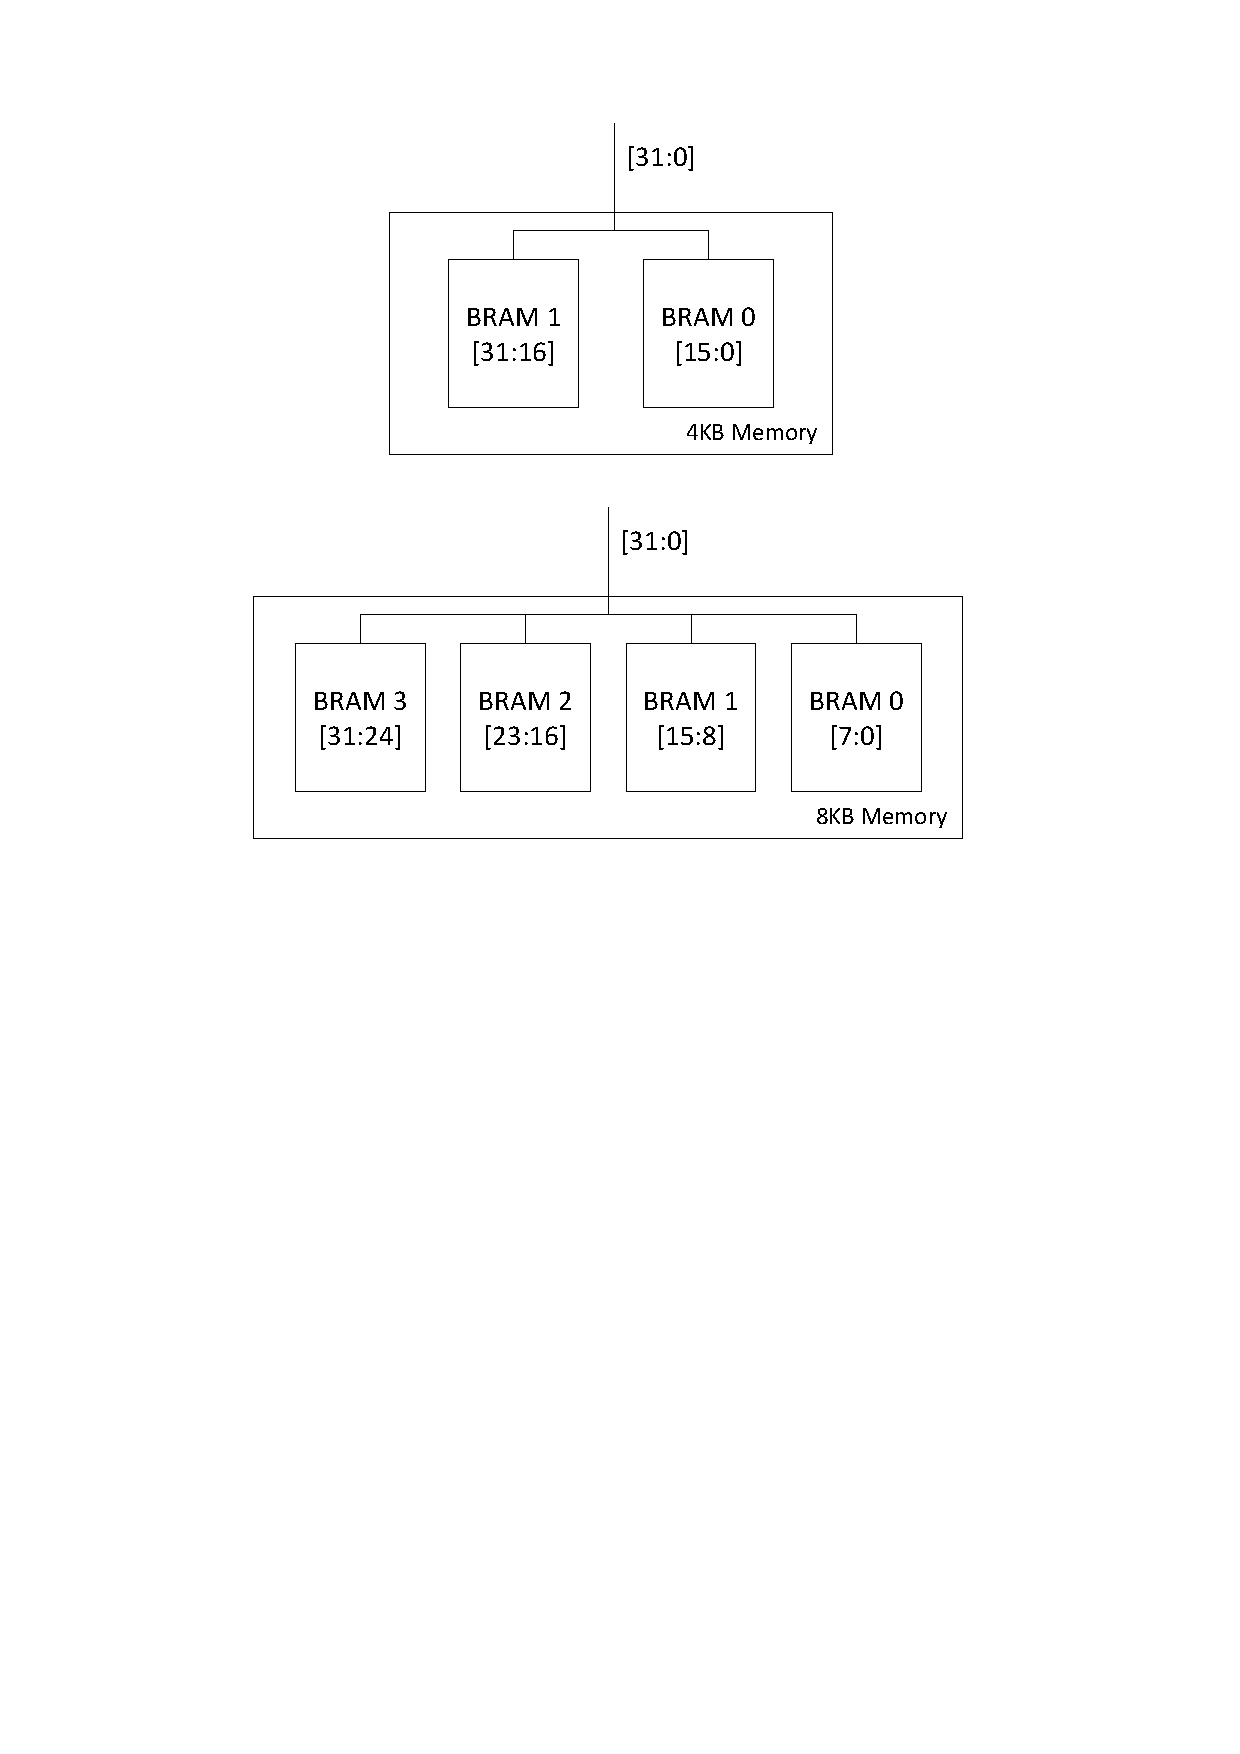
\includegraphics[width=0.7\linewidth]{./bilder/XilinxMEM}
\caption{Speicherstruktur der von Xilinx generierten Speichermodule}
\label{fig:XilinxMEM}
\end{figure}
In der Abbildung sind einfache Blockschaltbilder für einen 4KByte und einen 8KByte großen Speicher dargestellt. Angefangen bei einer Mindestgröße von 2KByte verdoppelt sich die Anzahl der Block RAMs bei jeder Vergrößerung. Dabei halbiert sich jeweils die Größe der Bitlanes bis hin zu einem Minimum von eins bei einer maximalen Speichergröße von 64KByte. Die vom XPS generierten Modelle instanziieren immer eine fixe Anzahl an Block RAMs, sodass es nicht möglich ist, mit der selben Methode wie beim Microblaze eine generische Parametriserbarkeit herzustellen. Daher muss, auf Grundlage der elaborierten Modelle, ein generisches Speichermodul geschrieben werden, dessen Größe über einen Parameter festgelegt werden kann.\\
Um dies zu erreichen, wird ein Verilog-Modul geschrieben, welches die Parameter \textit{RAMBLOCKS} und \textit{C\_FAMILY} hat. Über eine for-Schleife in einer generate-Umgebung werden entsprechend des Parameters \textit{RAMBLOCKS} dual-ported Block RAMS instanziiert. Einen Port handhabt Daten und der andere Instruktionen. Eine Funktion berechnet dabei aus dem Parameter die Breite der einzelenen Bitlanes. Um die Signalverbidungen zu realisieren, werden wires und regs deklariert, deren Größe mit \textit{RAMBLOCKS} skaliert. Über Indexing wird innerhalb der for-Schleife die Realisierung der einzelnen Bitlanes vorgenommen. Für das 4-Bit breite Write-Enable-Signal wird zusätzliche Kombinatorik hinzugefügt, da die Handhabung nicht durch einfaches Indexing umgesetzt werden kann.\\
Zuletzt werden der Speicher und zwei Speichercontroller in einer Top-Level-Beschreibung instanziiert und miteinander verbunden.

\subsection{Modulbeschreibungen} \label{subsec:Moduldesc}
Für den Microblaze, den Speicher, den UART-Core und den FSL-Core müssen nun XML-Modulbeschreibungen erstellt werden. Nachfolgend werden alle hierzu notwendigen Schritte besprochen:
\begin{itemize}
\item \textbf{Microblaze}: Der Microblaze wird in der Beschreibung als Prozessor kategorisiert. Neben den Wrapperdateien für den Microblaze, den LMBs und dem Reset-Modul müssen noch Pfadangaben für die HDL-Dateien der Implementationen dieser Cores angegeben werden. Um dies umzusetzen, wird die XML-Syntax mit \textit{externalRoot} um ein neues Konstrukt erweitert. Dieses Konstrukt erlaubt es absolute Pfade außerhalb des Default-Verzeichnisses anzugeben und wurde nicht im Rahmen dieser Arbeit ergänzt, sondern von einem Kommilitonen, der zum Zeitpunkt dieser Arbeit für die Wartung von JConfig verantwortlich war. Alle Dateien, die sich im Scope eines \textit{externalRoot}-Konstruktes befinden, verwenden den angegeben Pfad als Ausgangsverzeichnis. Im Rahmen dieser Arbeit, wurde in der Klasse \textit{HDLDescription} im Package \textit{de.tu\_darmstadt.rs.spartanmc.devxml.descriptions.generic} eine Anpassung vorgenommen, die Umgebungsvariablen in Pfadangaben auflöst. So wird über die Umgebungsvariable \textit{XILINX\_ROOT} plattformunabhängig der Pfad zu den HDL-Dateien angegeben. Desweiteren ist es möglich, einen Namen für eine VHDL-Library anzugeben, unter dem die entsprechenden Dateien zusammengefasst werden. Dies ist für die Xilinx Cores notwendig, da innerhalb der Implementationen einige Libraries referenziert werden. Außerdem verkürzen Libraries die Kompilierzeit während der Simulation.\\
Es folgen daraufhin die Angaben der Parameter. Hierbei wird darauf geachtet, dass die Gruppierung der Parameter in ähnlicher Weise erfolgt, wie es im Wizard des XPS der Fall ist. Die Parameter werden desweiteren mit einem Beschreibungstext versehen, sodass sich die Funktion für den Anwender bei der Parametrisierung erschließt. Außerdem haben die Konfigurationsmöglichkeiten einiger Parameter eine relativ geringe Aussagekraft. So lässt sich beispielsweise der Modus der MMU über einen Parameter steuern, der die Werte null bis drei annehmen kann. Um mehr Informationsgehalt zu vermitteln, wurde ein String-Parameter eingeführt, der die Werte \textit{``None''}, \textit{``Usermode''}, \textit{``Protection''} und \textit{``Virtual''} annehmen kann. Innerhalb der Top-Level-Verilog-Beschreibung wird dann über eine Aliasing-Funktion der String zu einem Integer umgewandelt. Dies wird für weitere Parameter durchgeführt, bei denen die Aussagekraft der Auswahlmöglichkeiten zu wenig Information vermittelt.\\
Desweiteren schließen sich einige Konfigurationsmöglichkeiten gegenseitig aus. So ist es beispielsweise nicht möglich, die MMU zu verwenden, wenn der Parameter \textit{C\_AREA\_OPTIMIZED} gesetzt ist. Um eine Auswahl in einem solchen Fall zu verhindern, wird das Konstrukt \textit{relevantIf} in Zusammenhang mit einer invertierten Version von \textit{C\_AREA\_OPTIMIZED} verwendet.\\
Darauf folgen Bus-Deklarationen für Speicherbusse und FSL-Busse (siehe \ref{subsec:BusDesc}), wie auch Signal-Deklarationen für Takt, Reset und dem AXI-Bus.\\
Abschließend wird das \textit{addressLayout} für den Daten- und Instruktionsspeicher definiert. Für Peripherie wurde noch kein Adressraum festgelegt, da es bis lang nur den UART-Core als Peripherie gibt, und dieser direkt mit dem Microblaze verbunden wird. Sobald ein AXI-Bus in JConfig verfügbar ist, muss auch ein Adressraum für die Peripherie hinzugefügt werden.
\item \textbf{Speicher}: Die Erstellung der Modulbeschreibung für den Speicher erfolgt ähnlich wie für den Microblaze. Die verfügbaren Parameter sind in Tabelle \ref{tab:MemParam} aufgelistet. Der Speicher wird allerdings als Memory kategorisiert und hat mit dem \textit{memory}-Konstrukt eine Besonderheit. Mit \textit{memory} wird die Größe des Speichers, das Namensschema der Speicherinstanzen und die Reset-Werte beschrieben. Außerdem kann angegeben werden, ob der Speicher eine Aufteilung zwischen Daten und Instruktionen vorsieht. Diese Informationen werden später bei der Erzeugung der Memory-Map benötigt.
\item \textbf{UART}: Auch hier wird die Modulbeschreibung nach ähnlichem Muster erstellt. Der UART-Core ist allerings als Peripherie kategorisiert. Über das \textit{registers}-Konstrukt können Angaben zu Registern innerhalb des Cores gemacht werden, die später während der Erstellung der Software verwendet werden können. Im Rahmen dieser Arbeit konnte dieses Konstrukt für die UART allerdings nicht mehr erstellt werden. Die zur Verfügung stehenden Parameter sind in Tabelle \ref{tab:UARTParam} zu finden.
\item \textbf{FSL}: Der FSL-Core wird als Core Interconnect kategorisiert und hat keine weiteren Besonderheiten. Die Parameter sind in Tabelle \ref{tab:FSLParam} aufgelistet.
\end{itemize}

\subsection{Busbeschreibungen}\label{subsec:BusDesc}
Um das Verbinden einzelner Komponenten zu vereinfachen, werden zusammengehörige Signale zu einem Bus zusammengefasst. Im Folgenden wird auf die, im Rahmen dieser Arbeit erstellten Busbeschreibungen eingegangen:
\begin{itemize}
\item \textbf{FSL-Busse}: Für den FSL-Bus werden zwei neue Busbeschreibungen in Form von XML-Dateien erstellt. Ein Bus beschreibt die Verbindungen für das Master-Interface und der andere die Verbindungen für das Slave-Interface (siehe Abbildung \ref{fig:FSLBSB}). Die Busbeschreibungen enthalten Defintionen für \textit{masterPorts} und \textit{slavePorts}, sowie alle dazugehörigen Signale, deren Richtung und Datenbreite.
Bei der Deklaration innerhalb der Modulbeschreibung für den Microblaze wird darauf geachtet, das die einzelnen Signale in den Busbeschreibungen mit der Option \textit{combineUsing="parallel"} versehen sind. Dies bewirkt, dass die einzelnen Signale, der bis zu 16 FSL-Busse konkateniert und so an den Microblaze weitergeleitet werden.
\item \textbf{Speicherbusse}: Sowohl alle für den Datenport des Speichers relevanten Signale, sowie alle für den Instruktionsport relevanten Signale, werden zu je einem Bus zusammengefasst. Die Beschreibung erfolgt nach ähnlichem Schema wie bei den FSL-Bussen. Die \textit{masterPorts} fassen alle Signale auf Seiten des Microblaze zusammen, während \textit{slavePorts} alle Signale des Speichers umfasst.
\end{itemize}
Für die AXI-Signale wurden im Rahmen dieser Arbeit noch keine Busse erstellt, dies sollte allerdings mit der Integration eines AXI-Bus-IP-Cores nachgeholt werden.

\section{Integration in die SpartanMC Toolchain}
\subsection{Ausgangslage}
Der Microblaze und alle notwendigen Peripherien sind in JConfig eingebunden. Mit den von JConfig generierten Dateien, kann die Toolchain allerdings noch kein funktionsfähiges Bitfile erzeugen, da die Speicherarchitekturen des SpartanMC und des Microblaze verschieden sind. Der Speicher des SpartanMC ist so aufgebaut, dass dem Parameter \textit{RAMBLOCKS} entsprechend Block RAMs instanziiert werden, dessen Bitlanes immer 18-Bit breit sind. So wird bei jedem Speicherzugriff auf genau ein Block RAM zugegriffen und nicht auf alle, wie es beim Microblaze der Fall ist.\\
Das Tool Initramj der SpartanMC Entwicklungsumgebung wird zur Speicherintialisierung für den SpartanMC verwendet und ist auf die vorher beschriebene Speicherstruktur angepasst. Das Tool ist unter anderem in der Lage, Speicherinitialisierungen in Form von UCF-Dateien, Verilog-Dateien oder Bitfile-Updates durchzuführen. Hierzu benötigt es eine ELF-Datei und eine Memory-Map in Form einer Datei namens \textit{memory.xml}. Es wäre also denkbar, Initramj dahingehend anzupassen, dass es auch die Speicherinitilaisierung für die 32-Bit-Speicherarchitektur des Microblaze durchführen kann. Dies hätte den Vorteil, dass die Speicherininitialisierung gekapselt von einem einzigen Tool gehandhabt würde und somit kaum Änderungen an den Makefiles notwendig wären.\\
Eine Alternative zu Initramj stellt die Speicherinitialisierung mit dem Xilinx-Tool data2mem dar. Hierfür müsste JConfig allerdings eine weitere Memory-Map in Form einer BMM-Datei erzeugen. Desweiteren müssten die Makefiles angepasst werden, sodass sie data2mem aufrufen. Im Rahmen dieser Arbeit wurde die Variante mit data2mem umgesetzt, da der Aufwand zur Anpassung von Initramj als zu hoch eingeschätzt wurde.\\
Desweiteren ist es notwendig, den Microblaze GCC in die Toolchain zu integrieren, da der SpartanMC Compiler keinen, vom Microblaze ausführbaren Code generieren kann. Um dies zu erreichen, müssen weitere Änderungen an den Makefiles vorgenommen werden.
\subsection{Erzeugung der BMM-Datei}
Damit JConfig in der Lage ist BMM-Dateien zu erzeugen, muss die Software erweitert werden. Das Package \textit{de.tu\_darmstadt.rs.spartanmc.jconfig.generation.outputProvider} des Tools libjconfig enthält diverse Klassen, welche auf Basis der, über das UI eingegebenen Informationen, die von der Toolchain benötigten Dateien generieren. An dieser Stelle wird eine neue Klasse namens \textit{BMMBuilderProvider} hinzugefügt. Diese Klasse generiert für jeden Speicher, der an einem Microblaze angeschlossen ist, einen Eintrag in der BMM-Datei, gemäß der Syntax, die in Abschnitt \ref{subsec:MemInitBMM} beschrieben ist. Das Namensschema für die Speicherinstanzen wird aus der XML-Modulbeschreibung des Speichers gewonnen. Um festzustellen, ob ein Speicher an einem Microblaze oder an einem SpartanMC angeschlossen ist, werden den XML-Modulbeschreibungen zwei virtuelle Parameter hinzugefügt (\textit{MB\_FLAG} für den Microblaze und \textit{SPMC\_FLAG} für den SpartanMC). Der \textit{BMMBuilderProvider} fügt einen Speicher nur dann zur Memory-Map hinzu, wenn der Parameter \textit{MB\_FLAG} vorhanden ist. Auf der anderen Seite muss aber auch verhindert werden, dass der Microblaze-Speicher in die \textit{memory.xml} aufgenommen wird, da Initramj ansonsten versuchen würden, eine Speicherinitialisierung für diese Module ebenfalls durchzuführen. Daher wurde die Klasse \textit{MemoryMapBuilderProvider} dahingehend angepasst, dass nur Speicher mit dem Parameter \textit{SPMC\_FLAG} hinzugefügt werden.\\
Damit JConfig die BMM-Datei auch erstellt, muss eine Instanz des \textit{BMMBuilderProvider} im Konstruktor der Klasse \textit{XilinxIseDocumentBuilder} hinzugefügt werden. Des weiteren werden die Dateien \textit{memory.xml} bzw. \textit{memory.bmm} nur dann erstellt, wenn auch ein SpartanMC bzw. ein Microblaze im System vorhanden ist.

\subsection{Anpassungen in der Toolchain zur Speicherinitialisierung}
Mit der BMM-Datei kann data2mem nun verwendet werden (auch wenn die ELF-Dateien mit dem Microblaze noch nicht konform sind, kann data2mem diese verwenden). Die einzelnen Anpassungen an den Makefiles werden im nachfolgenden beschrieben.
\subsubsection{Speicherinitialisierung mit UCF-Datei}
Die Speicherinitialisierung mit einer UCF-Datei findet statt, wenn ein Bitfile über die Regel \textit{``all''} erzeugt werden soll. Dabei wird eine weitere Regel namens \textit{\$(UCF)} aufgerufen, welche dafür sorgt, dass alle relevanten UCF-Dateien aktuell sind und diese dann über das Shell-Skript \textit{mkucf} zu einer Datei zusammengefasst werden. Um UCF-Dateien für Microblaze-Prozessoren einzubinden, wird eine neues Makefile mit dem Namen \textit{firmware\_mb.mk} erstellt, welches die Erzeugung der UCF-Dateien handhabt. Da data2mem pro Aufruf allerdings nur eine einzige Firmware behandeln kann, muss das Tool mehrfach aufgerufen werden. Hierzu wird eine \textit{for-each}-Schleife über alle Firmwares des Microblaze durchlaufen. Diese erzeugt für jede Firmware mit data2mem ein UCF-File. Um zu unterscheiden, welche Firmware zu welcher Prozessorart gehört, wird die Konstante \textit{JCONFIG\_FIRMWARE\_IDS} aus dem, von JConfig generierten Makefile \textit{firmwares.mk} aufgeteilt in \textit{JCONFIG\_SPARTANMC\_FIRMWARE\_IDS} und \textit{JCONFIG\_MICROBLAZE\_FIRMWARE\_IDS}. Die hierzu notwendigen Änderungen an der Software werden in der Klasse \textit{LegacyMkBuilderProvider} vorgenommen.\\
Die so erstellten UCF-Dateien werden an das Shell-Skript \textit{mkucf} übergeben, welches daraus eine einzelne Datei macht. Die Syntax für den Aufruf von data2mem ist wie folgt:\\\\
\indent
\textit{data2mem -bm <BMM-Datei> -bd <ELF-Datei> tag <Prozessorname> -o u <UCF-Datei>}\\\\
Die Option \textit{-bm} spezifiziert die BMM-Datei und \textit{-bd} die ELF-Datei. Der Zusatz \textit{tag} ist notwendig, um die zum Prozessor passende \textit{ADDRESS\_MAP} in der BMM-Datei zu spezifizieren und \textit{``-o u''} gibt an, dass das Ausgabeformat eine UCF-Datei sein soll. Mit der UCF-Datei können während der Synthese die Block RAMs initialisiert werden.
\subsubsection{Aktualisierung des Bitfiles}
Die Speicherinhalte eines bestehenden Bitfiles werden beim Aufruf der Regel \textit{bitgen} erzeugt. Um die Updates für die Speicher des Microblaze durchzuführen, wird in die Liste der Prerequisites eine neue Regel namens \textit{bit\_mb\_update} hinzugefügt. Diese Regel ruft für jede Firmware eines Microblaze data2mem auf und aktualisiert das Bitfile. Für die Aktualisierung des Bitfiles benötigt data2mem allerdings eine BMM-Datei, die Placement-Informationen der Speicherinstanzen beinhaltet. Diese Datei kann allerdings von der Xilinx Toolchain erzeugt werden, wenn dem Translate-Tool NGDBuild beim Aufruf die originale BMM-Datei mit der Option \textit{-bm} übergeben wird. Die Syntax für den Aufruf von data2mem ist wie folgt:\\\\
\indent
\textit{data2mem -bm <BMM-Datei> -bd <ELF-Datei> tag <Prozessorname>\\
\indent \indent \indent -bt <zu aktualisierendes Bitfile> -o b <neues Bitfile>}
\subsubsection{Speicherintialisierung für die Simulation}
Die Speicherinitialisierung für die Simulation wird mittels Verilog-Dateien durchgeführt. Durch ausführen der Regel \textit{sim} wird eine entsprechende Verilog-Datei von Initramj erzeugt. Durch hinzufügen einer Regel in dem Makefile \textit{firmware\_mb.mk} wird durch Aufruf von data2mem für jede Firmware eine Verilog-Datei erzeugt, die die Speicherinitialisierung enthält. Der Aufruf hierfür ist ähnlich, wie bei der Erzeugung der UCF-Dateien:\\\\
\indent
\textit{data2mem -bm <BMM-Datei> -bd <ELF-Datei> tag <Prozessorname> -o v <Verilog-Datei>}\\\\
Die so erzeugten Verilog-Dateien müssen nun noch zusammengefasst werden, da innerhalb der automatisch erzeugten Testbench nur ein einziges Initialisierungsmodul instanziiert wird. Es könnte auch eine Anpassung der Software vorgenommen werden, die für jede erzeugte Verilog-Datei eine Instanz in der Testbench erzeugt. Das Zusammenfassen der einzelnen Dateien stellt allerdings die elegantere Lösung dar und wird deshalb umgesetzt. Hierzu wurde ein Shell-Skript namens \textit{mksim} auf Basis des Skripts \textit{mkucf} erstellt. Es erhält als Eingabe eine unbestimmte Anzahl an Verilog-Dateien (sowohl für SpartanMC als auch Microblaze) und fügt diese zu einer einzigen Datei zusammen. Dabei werden noch zwei Zeilen eingefügt, die die Speicherinitialisierung als Verilog-Modul definieren (die entsprechenden Zeilen werden bei der Datei für den SpartanMC vorher entfernt). Außerdem wird der hierarchische Name der Speicherinstanzen, als Konsequenz aus der Initialisierung innerhalb der Testbench, um das Präfix \textit{``UUT.''} erweitert.\\
Der Aufruf des Skripts findet innerhalb der Regel \textit{sim} statt.

\subsection{Unterstützung von Libraries in der Simulation}
In Abschnitt \ref{subsec:Moduldesc} wurde bereits darauf eingegangen, dass Xilinx IP-Cores VHDL-Libraries referenzieren. Einer der Vorteile von Libraries ist, dass alle Dateien innerhalb einer vorkompilierten Library bei erneutem Kompilieren nicht berücksichtigt werden und daher Zeit gespart wird. Xilinx bietet mit dem Tool compxlib eine Möglichkeit Simulationslibraries für sämtliche IP-Cores des EDK zu erstellen. Die Auswahlmöglichkeiten bei der Erzeugung sind allerdings eingeschränkt. So ist es nicht möglich einzelne IP-Cores zu kompilieren, sondern es werden Simulationsmodelle für alle Cores des EDK erstellt. Der hierfür verwendete Speicherplatz ist mit mehr als 2GByte verhältnismäßig groß. Daher werden nur die Simulationslibraries der Hardware behalten, welche in JConfig eingebunden wurde. Die Auswahl wird mit einer Größe von ca. 70MByte dem SpartanMC Git-Repository in dem Verzeichnis \textit{``spartanmc/simLib''} hinzugefügt, um zu gewährleisten, dass Nutzer die Libraries nicht selbst kompilieren müssen.\\
Um die neuen Libraries in der Simulation einzubinden, müssen Anpassungen an dem Skript \textit{configure.tcl} vorgenommen werden. Hierzu benötigt das Skript Informationen darüber, welche Libraries eingebunden werden müssen und wo diese zu finden sind. In der Klasse \textit{XilinxIseProjectBuilderProvider} wird dazu ein neues Makefile namens \textit{sim\_lib.mk} erzeugt, welche eine Liste aller benötigten Libraries definiert. Desweiteren wird die Erstellung des Do-Skripts \textit{spartanmc\_worklib.fdo} angepasst, welche Befehle zur Kompilierung aller notwendigen Dateien enthält, sodass Dateien innerhalb einer Library nicht hinzugefügt werden, da diese ja vorkompiliert sind. Um die Pfadangabe zu den Simulationslibraries zu realisieren, wird in JConfig der Konfiguration unter dem Reiter Target das Feld \textit{Simulation Library Path} hinzugefügt. Diese Pfadangabe wird im Makefile \textit{project.mk} unter der Konstanten \textit{JCONFIG\_SIMULATION\_LIBRARY\_PATH} abgelegt. Mit diesen Informationen kann das Skript \textit{configure.tcl} die entsprechenden Libraries hinzufügen. Des weiteren wurden noch Mappings für die Libraries \textit{ieee}, \textit{std} und \textit{synopsys} ergänzt, da diese ebenfalls benötigt werden.
\subsection{Integration des Microblaze GCC}
Die Integration des Microblaze GCC konnte im Rahmen dieser Arbeit aus zeitlichen Gründen nicht durchgeführt werden. Es wird an dieser Stelle allerdings kurz darauf eingegangen, welche Ansätze für die Integration vorstellbar wären.\\
Die für den Ablauf des Build-Prozesses verwendeten Makefiles sind, ausgehend vom SpartanMC Root-Verzeichnis, unter dem Pfad \textit{``src/scripts/make/firmware/''} zu finden. Das Makefile \textit{fwbuild-gcc.mk} ist dabei für die Erzeugung der Firmware verantwortlich. Hierzu erstellt es auf Basis des Templates \textit{gcc-build.mk} (zu finden im Verzeichnis \textit{``templates''}) je ein Makefile für jede Firmware. Diese erzeugten Makefiles beinhalten alle notwendigen Regeln, um eine ELF-Datei zu erzeugen. In \textit{fwbuild-gcc.mk} werden desweiteren alle verwendeten Tools, Source-Dateien und Flags für Compiler, Assembler und Linker festgelegt. Um den Microblaze GCC zu integrieren sollten in dieser Datei Änderungen vorgenommen werden.\\
Der Microblaze GCC und die Binutils sind im Xilinx ISE Installationsverzeichnis unter folgendem Pfad zu finden: \textit{``14.7/ISE\_DS/EDK/gnu/microblaze/lin/bin/''}. Desweiteren müssen basierend auf der Konfiguration des Microblaze bestimmte Compiler-Flags gesetzt werden, um Hardwarebeschleuniger zu integrieren. Hierzu ist es notwendig, dass die Software erkennt, wenn ein entsprechender Parameter gesetzt ist und das dazugehörige Flag in dem Makefile \textit{firmwares.mk} hinzufügt. Relevante Informationen zum GCC sind im \textit{Embedded System Tools Reference Manual} Kapitel 9 zu finden \cite{MGNU}.\\
Außerdem müssen entsprechend der verwendeten Hardware passende Treiber inkludiert werden. Die Software zur Verwendung von Xilinx IP-Cores ist unter folgendem Pfad zu finden: \textit{``14.7/ISE\_DS/EDK/sw/XilinxProcessorIPLib/drivers/''}.
\chapter{Implementierung}

\begin{lstlisting}
inst "subsystem_0/spartanmc_0/ifid/memory/MEM_BL[0].DPRAMA"
 INITP_00::d8aa100063c47860a000003c49c07832c10491802825301224b24c5014400024
 INITP_01::0000030048018d68a923f02b84b0d9462112c00611594c22a96186c986d31e03
  INIT_00::000035a500a4011000a000000000000000000000000000002015221600051f00
  INIT_01::8015648415fe0880ff1564884600863f0084370080822200016401ff1f9e012c
  INIT_02::1525500040009d001514ff8000fe156401156485a0821507018015648215fe01
  INIT_03::dfff800001001505c50215251525a505ff811564020015f6ff8000010015e50e
  INIT_04::01a580156401156490b00390850615ac0985ffd0811015ac0985ffd08085e915
  INIT_05::6480bc016715736415787015752d15ec6f7e156f30011815ec09ffd085ffc080
  INIT_06::62ceeb15ec09ffd085ffc08001da15ec09ffd085ffc080012085bdc534153015
  INIT_07::85ffc08587c58002a5156480b601cb1525154bd015ac583415582d15ec625115
  INIT_08::855504a515648542e5c5a5a815649bc330ec09ffd085ffc080013915ec09ffd0
  INIT_09::6d308280bc0180ff1564853f01a51564854503a51564856fe5c5a51564a51564
  INIT_0A::8506c5ff00a5156415c58582842200ff15640015fbff800115a55000150bff80
  INIT_0B::00139300000e00ffa401e5ffc51564a5f385ac1a008c2d0e0031019f15648537
  INIT_0C::2030001b00ce01c5ff1564853521001564853bf58000a6e0f0be01d485ffff21
  INIT_0D::41004030e315d8d80102ff0115044005f8ff8a9085f08501013092019f10408a
  INIT_0E::31b8003fb400000a216c6f206c651564fb150080ffff04ff15648504ffa51b00
INIT_0F::00000000000000000000000000000000000000010a64e810a046444239373533 ;
\end{lstlisting}

\chapter{Benutzungshinweise}
Um die Verwendung des Microblaze in der SpartanMC Entwicklungsumgebung zu erklären, wird an dieser Stelle Stück für Stück ein einfaches \textit{"Hello World!"}-Beispiel erstellt.
Hierzu wird zunächst ein neues SpartanMC-Projekt angelegt und JConfig gestartet. Der erste Schritt ist es, den Microblaze Prozessor hinzuzufügen. Der Prozessor ist unter \textit{``Subsystem modules --> Processors --> Microblaze core''} zu finden. Als nächstes wird ein Speichermodul für den Microblaze hinzugefügt, welches unter \textit{``Common modules --> Memory --> Microblaze Local Memory''} zu finden ist. Zur Ausgabe des Strings \textit{``Hello World!''} wird noch ein UART-Core benötigt. Dieser findet sich unter \textit{``Peripheral modules --> Bus --> AXI UART Light''}. Die Parametrisierung für die eingebunden Komponenten wird, bis auf die Baudrate der UART nicht verändert. Diese wird auf 115200 gestellt, um in der Simulation nicht lange auf Ergebnisse warten zu müssen. Zuletzt wird noch ein Modul zur Takterzeugung eingebunden, welches unter \textit{``Common modules --> Clocks --> Xilinx DCM Clock''} zu finden ist. An der Konfiguration des Taktmoduls wird ebenfalls nichts verändert.\\
Der nächste Schritt ist das Verbinden der Signale. Beim Betrachten der Verbindungen wird festgestellt, dass der Microblaze bereits mit dem Speicher- und Takterzeugungsmodul verbunden ist. Das Signal \textit{reset} muss noch mit dem Pin, der das Reset-Signal führt, verbunden werden (für das SP601 ist dies N4). Desweiteren müssen die AXI-Signale mit den gleichnamigen Signalen des UART-Cores verbunden werden. Bei den Adresssignalen muss eine partielle Verbindung erstellt werden. Der UART-Core wird noch mit dem Taktsignal und dem Reset-Signal \textit{peri\_resetn} des Microblaze verbunden. Das TX-Signal muss auf dem SP601 mit dem Pin K14 verbunden werden und das RX-Signal mit L12.\\
Desweiteren ist für die Konfiguration unter dem Reiter \textit{Target} in das Feld \textit{Simulation Library Path} der absolute Pfad zu den Simulationslibraries einzugegeben. Das erstellte System ist in Abbildung \ref{fig:ExampleSystem} zu sehen.

\begin{figure}[th!]
\centering
\includegraphics[width=1\linewidth]{./bilder/ExampleSystem}
\caption{\textit{"Hello World!"} Beispielsystem}
\label{fig:ExampleSystem}
\end{figure}
\noindent
Bevor die für die Toolchain relevanten Dateien erzeugt werden können, muss zunächst eine Dummy-Firmware erzeugt werden. Hierzu wird der Befehl \textit{make newfirmware +path=<path-to-firmware>} verwendet. In der Verzeichnisstruktur muss im Ordner \textit{src} eine Datei namens \textit{main.c} hinzugefügt werden. In dieser Datei muss eine Funktion namens \textit{main} implementiert sein. Der Inhalt dieser Funktion ist egal, da der Microblaze GCC noch nicht in die Toolchain integriert ist und die Speicherintialisierung manuel durchgeführt wird. Für dieses Beispiel soll folgender Code verwendet werden. Im Anschluss wird in JConfig auf \textit{Build All} geklickt um die Dateien zu erzeugen.
\begin{lstlisting}
#include <subsystems/microblaze_spmc_0/peripherals.h>
#include <stdio.h>
void main() {
	while(1){
		printf("hello world\n");
	}
}
\end{lstlisting}
Für den Fall, dass das Beispielsystem mit Hardware verwendet werden soll, muss nun eine Bitfile mit \textit{make all} generiert werden. Im Verzeichnis \textit{``spartanmc/hardware/microblaze/example''} ist eine ELF-Datei namens \textit{hello\_world.elf} zu finden. Diese enthält ausführbaren Code für ein einfaches, dem oben beschriebenen SoC sehr ähnlichem System. Die ELF-Datei beschreibt ein simples \textit{"Hello World!"} Programm. Mit data2mem wird nun das Bitfile manuel aktualisiert. Der Aufruf ist wie folgt:\\\\
\indent
\textit{data2mem -bm memory\_bd.bmm -bd hello\_world.elf tag microblaze\_spmc\_0\\
\indent \indent \indent -bt spartanmc.bit -o b spartanmc.bit}\\\\
Danach kann mit \textit{make program} das Bitfile auf das FPGA gespielt werden.\\
Für den Fall, dass das Beispielsystem simuliert werden soll, muss zunächst eine Speicherinitialisierung in Form einer Verilog-Datei erzeugt werden. Dazu ist folgender Aufruf von data2mem notwendig:\\\\
\indent
\textit{data2mem -bm memory.bmm -bd hello\_world.elf tag microblaze\_spmc\_0 -o v sim1.v}\\\\
Im selben Verzeichnis in dem sich die ELF-Datei befindet, existiert ein Shell-Skript namens \textit{mksim}, welches die Verilog-Datei für die Simulation präpariert. Der entsprechende Kommandozeilenbefehl ist folgender:\\\\
\indent \textit{sh mksim sim1.v}\\\\
Dadurch wird die Datei \textit{init\_ram.v} erstellt. Diese Datei wird im SpartanMC-Projekt im Verzeichnis \textit{build} abgelegt. Nun muss noch der Eintrag \textit{spartanmc\_sim.v} in der Datei \textit{system/spartanmc\_worklib.fdo} in \textit{init\_ram.v} umgeändert werden. Als nächster Schritt folgt das Erzeugen eines Simulationsverzeichnisse mit dem Befehl \textit{make newsim +path=<path-to-sim>} und abschließend das Starten der Simulation im neuen Verzeichnis mit \textit{vsim -do testbench.fdo}. Der Simulatior sollte starten und das System kann simuliert werden. 
\chapter{Evaluation}
\begin{itemize}
\item \textbf{Änderungsmöglichkeiten kleinerer Art}
\begin{itemize}
\item[-] Löschen einer Funktion
\item[-] Hinzufügen einer Funktion
\item[-] Umbenennen einer Funktion
\item[-] Ändern des Körpers einer Funktion 
\end{itemize}
\end{itemize}
Diese Änderungen kleinerer Art führten bei meiner Programmierung zu korrekten Ergebnissen.
\begin{itemize}
\item \textbf{Funktionalitätsänderungen}
\begin{itemize}
\item[-] Ein kleines Programm in ein großes Programm ändern.
\item[-] Ein großes Programm zu einem anderen großen Programm ändern.
\item[-] Ein großes Programm in ein kleines Programm ändern.
\end{itemize}
\end{itemize}

\chapter{Ausblick}

\chapter{Zusammenfassung}


\section*{Abkürzungsverzeichnis}
\begin{acronym}
 \acro{CPU}{Central Processing Unit}
 \acro{MC}{Microcontroller}
 \acro{FPGA}{Field Programmable Gate Array}
 \acro{SoC}{System on Chip}
 \acro{I/O}{Input/Output}
 \acro{UART}{Universal Asynchronous Receiver Transmitter}
 \acro{IP}{Intellectual Property}
 \acro{FSL}{Fast Simplex Link}
 
 \acro{NCD}{Native Circuit Description Format}
 \acro{SoC}{System on Chip}
 \acro{Sph}{SpartanMC Hex Dateiformat}
 \acro{XDL}{Xilinx Design Language Format}




\end{acronym}

\listoffigures
\listoftables
\clearpage

\makeatletter
\renewcommand\chapter{\thispagestyle{\chapterpagestyle}%
                    \global\@topnum\z@
                    \@afterindentfalse
                    \secdef\@chapter\@schapter}
\makeatother

\nocite{*}
\bibliographystyle{alphadin}
\bibliography{Literaturverzeichnis}

\end{document}